%%% Third chapter

\chapter{Third Chapter}

\lipsum[23-30]

\section{First Section}

\lipsum[33]

\begin{table}[!ht]
	\begin{center}
		\caption{Continent sizes}
		\index{continents}
		\label{tab2}
        \begin{tabular}{lr}
	       \rowcolor{Moccasin} \multicolumn{2}{c}{\bfseries Continental Areas {\small(sq. mi.)}}\\
	       \hline
           Asia    & 17,212,000\\
	       Africa  & 11,608,000\\
	       North America  & 9,365,000\\
	       South America  & 6,880,000\\
	       Antarctica     & 5,100,000\\
	       Europe         & 3,837,000\\
	       Australia      & 2,967,908\\
        \end{tabular}
	\end{center}
\end{table}

\section{Second Section}

\lipsum[34]

\begin{figure}[!ht]
	\begin{minipage}{5.9in}
		{\mdseries\footnotesize\textsf{\hspace{19.25em}Map courtesy of Library of Congress free-to-use images.}}
		\begin{center}
			{\vspace{-1.5ex}}
			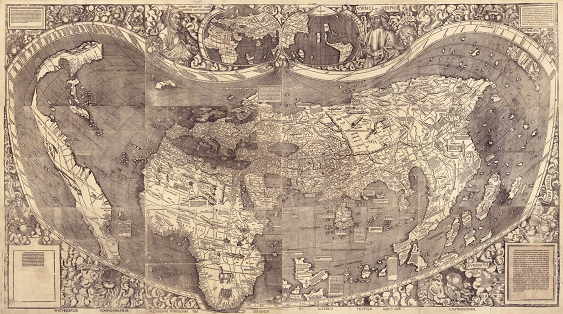
\includegraphics[width=0.85\linewidth]{world_map3}
			\caption{Cartograph}
			\label{fig:map3} 
		\end{center}
	\end{minipage}
\end{figure}